\subsection{Grep}\label{sec:grep}

We implemented a generic module, GrepModule, that selects a fraction of the records in a dataseries file based on a user-specified ``matcher" function that determines whether a specific record should be preserved. We implemented an analysis program, grepanalysis, that uses GrepModule to implement a tool similar to the UNIX grep utility. This analysis simply selects the records that contain a user-specified substring.

For the experiment, we downloaded a text version of The Bible and concatenated it multiple times to create three files of approximately the following sizes: 100 MiB, 1 GiB and 10 GiB. We then converted these text files to DataSeries files with one record for each line of text (where each record consists of a single variable32 field). For each of the three datasets, we created three distinct DataSeries files: one without compression, one with lzf~\cite{LZF} compression and one with gzip~\cite{GZIP} compression.

The effective throughput (ie, uncompressed bytes/s, or records/s) of the analysis program was significantly higher with compressed input. On the 1 GiB files, for example, the analysis program had 0.87$\times$ the throughput of UNIX grep on the uncompressed dataset, and 1.7$\times$ and 2.66$\times$ the throughput of UNIX grep on the lzf and gzip datasets, respectively.

\subsubsection{Conversion to DataSeries}

The conversion to DataSeries was straightforward. We implemented a simple utility, txt2ds, which convers a text file to a DataSeries file by creating one record for each line of the text file. The record consists of a single variable32 field. The txt2ds tool allows the user to specify the desired compression algorithm.

Table~\ref{table:grep:compression} shows the sizes of each of the datasets in four different formats: the original text file, the uncompressed DataSeries format, the lzf DataSeries format and the gzip DataSeries format.


\begin{table*}
\centering
\begin{tabular}{|l|r|r|r|}\hline

Dataset           & 35 copies & 350 copies  & 3500 copies \\
\hline
Text              & 100.84 & 1008.40 & 10084.10   \\
DS/none           & 111.08 & 1110.80 & 11108.03   \\
DS/lzf            & 55.50  & 555.02  & 5550.26    \\
DS/gz             & 34.21  & 342.11  & 3421.11    \\
\hline
\end{tabular}


\caption{File sizes (MiB) for the three datasets (35, 350 and 3500 copies of The Bible) using different compression algorithms. The overhead of the DataSeries format (and variable32 fields, specifically) caused the uncompressed DataSeries files to be 1.102$\times$ the size of the original text files. However, compression resulted in significantly smaller files. Specifically, the lzf files were 0.55$\times$ the size of the original text files, and the gzip files were 0.34 times the size of the original text files.}

\label{table:grep:compression}
\end{table*}

\subsubsection{Experiments}

For each of the datasets, we ran our analysis program on each of the three DataSeries formats (no compression, lzf and gzip). Table~\ref{table:grep:runtime} shows the runtime of these experiments, and Figure~\ref{fig:grep:throughput} shows the effective throughput. Since string searching is not computationally intensive, we expected disk throughput to be the performance bottleneck, and indeed reducing the file sizes via compression increased the throughput. 

To observe the rate at which data was read from the disk, we can divide the actual (ie, after compression) file size by the runtime. For the 1 GiB dataset, the rate was 106.18, 101.69, 99.58 and 95.65 MiB/s (UNIX grep, DataSeries with no compression, DataSeries with lzf compression and DataSeries with gzip compression), indicating that DataSeries' unpacking and decompression hardly reduced the disk throughput. Therefore, the effective throughput was almost linear in the compression ratio (179.43 MiB/s for lzf and 279.56 MiB/s for gzip), resulting in a much higher effective throughput than the UNIX grep utility.

\begin{table*}
\centering
\begin{tabular}{|l|r|r|r|}\hline

Dataset     & 35 copies (100 MiB) & 350 copies (1 GiB)  & 3500 copies (10 GiB) \\
\hline
Text        & 1.06  & 9.50  & 96.83     \\
DS/none 	& 1.35  & 10.92 & 112.56    \\
DS/lzf      & 0.77  & 5.57  & 60.43     \\
DS/gz       & 0.62  & 3.58  & 36.04     \\
\hline
\end{tabular}

\caption{Average runtime of UNIX grep and grepanalysis.}

\label{table:grep:runtime}
\end{table*}

\begin{figure}
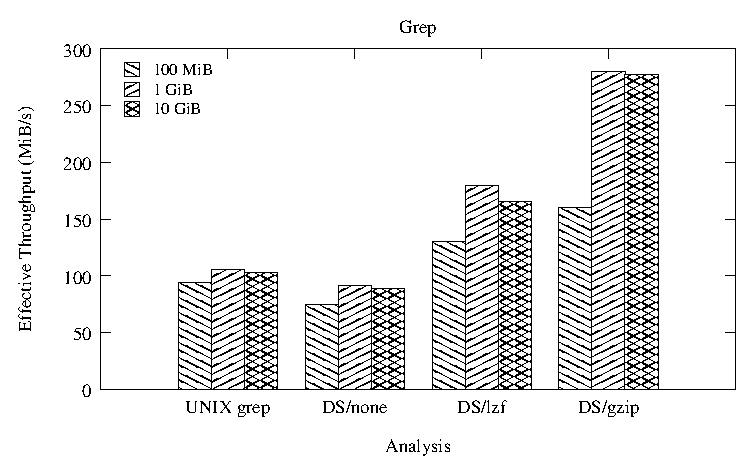
\epsfig{width=3.2in, angle=0, file=graphs/grep.ps}
\caption{Throughput of string searching with DataSeries. String searching is not I/O-bound, so the effective throughput can be increased via compression. Our DataSeries-based analysis was slower than the popular UNIX grep utility when we did not use any compression, but faster we did use compression. For the 10 GiB dataset, using gzip compression resulted in 2.87$\times$ the throughput of UNIX grep.}
\label{fig:grep:throughput}
\end{figure}

